\documentclass[a4paper,12pt]{article}


% add more packages if necessary
\usepackage{xspace}
\usepackage[utf8]{inputenc}
\usepackage{graphicx}
%\usepackage{xcolor}
%\usepackage{hyperref}

\usepackage{color}
\definecolor{orange}{rgb}{1,0.5,0}
\definecolor{lightgray}{rgb}{.9,.9,.9}
\definecolor{bluekeywords}{rgb}{0.13,0.13,1}
\definecolor{greencomments}{rgb}{0,0.5,0}
\definecolor{redstrings}{rgb}{0.9,0,0}


% TODO: Add your group name
\newcommand{\groupname}{Tortoise\xspace}


\title{
Project Report \\ 
Group \groupname \\
\vspace{5mm}
\large Java and C\# in depth, Spring 2014
}
\author{
% TODO: Add your names here
Lukas Häfliger\\
Fabian Meier\\
Andrea Canonica
}
\date{\today}

% code listings

\usepackage{listings}
\lstset{language=[Sharp]C,
showspaces=false,
showtabs=false,
breaklines=true,
showstringspaces=false,
breakatwhitespace=true,
numbers=left,
captionpos=b,
morekeywords={\#if, \#endif, \#else},
escapeinside={(*@}{@*)},
commentstyle=\color{greencomments},
keywordstyle=\color{bluekeywords}\bfseries,
stringstyle=\color{redstrings},
basicstyle=\ttfamily
}




\begin{document}
\maketitle

%\section{Introduction}

%This document describes the design and implementation of the \emph{Personal Virtual File System} of group \emph{\groupname}. The project is part of the course \emph{Java and C\# in depth} at ETH Zurich. The following sections describe each project phase, listing the requirements that were implemented and the design decisions taken. The last section describes a use case of using the \emph{Personal Virtual File System}.

% PART II: VFS Browser
% --------------------------------------

\section{Client and Server}

For this part of the project we made two new user interfaces, a client interface and a server interface. On startup, the user can choose in which mode the application should run. If he chooses "Client", a simple dialog will open where he can specify the IP and port of the server, as well as his login. If the connection is successful he can open an Explorer Window (which is the same as in part 2) or he can choose to work offline. \\
If the application is started as a server, a new server window opens. Here the administrator can start and stop the server and register new users. All registered users are displayed on a list which also indicates the online state of a user. On the right side a log is displayed which lists all transactions. \\

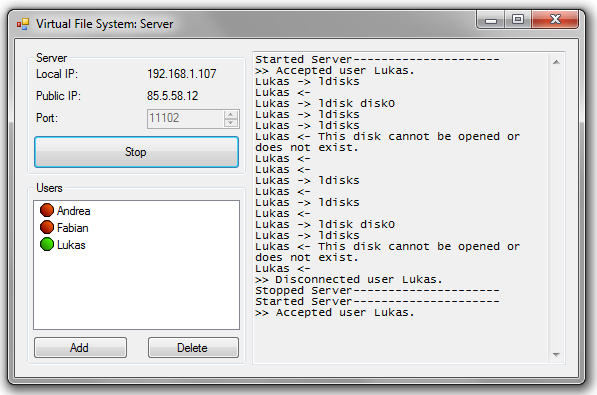
\includegraphics[scale=0.8] {servergui}

\subsection{Design}

This part of the project builds directly on the two previous parts (which we separated into their own assemblies, thus they both still run independently). Since in part 2, the interface between the \emph{VfsExplorer} and the \emph{VfsManager} (part 1) was already designed very narrow, the step into a distributed environment was reasonably easy. In the graphic below you see that the manager and explorer were only connected by the classes \emph{LocalConsole} and \emph{RemoteConsole}, which only communicate command line like strings. To introduce networking we added the two classes \emph{LocalConsoleAdapter} and \emph{RemoteConsoleAdapter}, which are subclasses of the corresponding Console-classes. These two classes mainly contain networking code to send messages, which originally were console in- and outputs, to each other. To control this new setup we also added a \emph{VfsClient} and a \emph{VfsServer} GUI. \\
The distribution of the VFS is organized as follows:

\begin{itemize}
\item The server has a copy of all virtual disks locally. when a user commits a command it will be queued into the VFS and then executed. If it was successfull, the command is sent back to all machines of the same user.
\item Each machine of a user has its own local copy of a disk. An issued command is first sent to the server, and it is only locally applied if the server sends it back. This prevents race conditions between simultaneous commands.
\item Import and export commands are treated separately, since they require more communication than just the basic string messages.
\end{itemize}


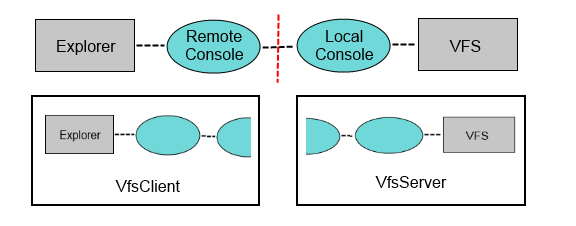
\includegraphics[scale=0.8] {design}


\subsubsection{VfsServer}
This class is a GUI which allows the administrator to set up a server. It initiallizes a new manager instance and connects it's \emph{LocalConsole} to a new \emph{RemoteConsoleAdapter} instance. The manager was not modified for this environment and still works the same way as before.
\subsubsection{RemoteConsoleAdapter}
This class represents the server-side network interface. When the adiministrator starts the server, it opens a new TCP listener and accepts incoming client connections. All of the serverside encoding and decoding of messages is handled by this class.
\subsubsection{VfsClient}
This class is the client GUI which users use to connect to the server. When the user starts a connection attempt, this class starts a new \emph{LocalConsoleAdapter} instance. If the connection is succesful and the user clicks the "Explorer" button this class creates and shows  a new \emph{VfsExplorer} and connects it's \emph{RemoteConsole} to the new \emph{LocalConsoleAdapter}. The explorer required almost no modification to work in this mode, only one Boolean indicator to handle the adding of new disks.
\subsubsection{LocalConsoleAdapter}
This class handles the client-side of the network interface. All of the clientside encoding and decoding of messages is handled by this class.

\subsubsection{Networking Messages}
We defined 10 network message types used for this project. The Message type is encoded as the first Byte of the sent data. Most messages contain only an encoded string after that, except the File Transfer messages, which also contain a whole file. To reduce bandwith usage we restrict import and export of files larger than 4MB in this mode.
\begin{itemize}
\item Wrong User or Password
\item Accept User
\item Command
\item Success Message
\item Error Message
\item Query
\item File Transfer (import)
\item File Transfer (export)
\item End
\end{itemize}


\subsection{Requirements}
Our VFS Network provides the following features:

\subsubsection{Server}

\begin{itemize}
\item \textbf{The browser should allow the user to create a new account or to log in to an existing account.} \\
	The client GUI allows a user to log in, but we restricted registration to the server, since a user should not be able to add himself.
\item \textbf{ The browser should offer to switch to an offline mode, and be able to operate without a connection
to the server.} \\
	The client GUI has a botton "Work Offline" which allows opening all local disks.
\item \textbf{The browser should support linking an existing virtual disk to an active account. (Partial)} \\
	Disks are synchronized over multiple machines.
\end{itemize}

\subsubsection{Client}

\begin{itemize}
\item \textbf{ The server should support registration of unique accounts. Each account is identified by name and password.} \\
	Users can be registered and their passwords can be set.
\item \textbf { The server should track changes to linked virtual disks of registered accounts and synchronize
changes across machines hosting linked disks.}
	Disks are synchronized over multiple machines.
\item \textbf{A concurrent client/server system (Bonus feature)}
	Our Network system allows concurrent modifications and updates to the explorer happen after each user interaction.
\end{itemize}

\end{document}




























